% MICRO 2026 Survey Paper - ML Performance Models
% Using MICRO 59 ACM sigconf template
% Last compiled: 2026-02-07 (rebuild triggered)

%%
%% For submission and review of your manuscript please change the
%% command to \documentclass[manuscript, screen, review]{acmart}.
%%
\documentclass[sigconf, screen, review]{acmart}

%%
%% \BibTeX command to typeset BibTeX logo in the docs
\AtBeginDocument{%
  \providecommand\BibTeX{{%
    Bib\TeX}}}

%% Rights management information - for submission
\setcopyright{none}
\copyrightyear{2026}
\acmYear{2026}
\acmDOI{}

%% Conference information
\acmConference[MICRO 2026]{The 59th IEEE/ACM International Symposium on Microarchitecture}{November 2026}{Austin, TX, USA}
\acmISBN{}

%% Disable ACM reference format printing for submission
\settopmatter{printfolios=true}
\settopmatter{printacmref=false}

%% Anonymous submission
\author{Anonymous Author(s)}
\affiliation{%
  \institution{Under Review}
  \country{Anonymous}
}

%% Additional packages (acmart already loads amsmath, amsfonts, amssymb, booktabs)
\usepackage{multirow}
\usepackage{tikz}
\usetikzlibrary{shapes.geometric,arrows.meta,positioning,fit,backgrounds,patterns,decorations.pathreplacing}
\usepackage{pgfplots}
\pgfplotsset{compat=1.18}
\usepgfplotslibrary{groupplots}
\usetikzlibrary{plotmarks}

% Custom commands
\newcommand{\todo}[1]{\textcolor{red}{[TODO: #1]}}

\begin{document}

\title{A Survey of High-Level Modeling and Simulation Methods for Modern Machine Learning Workloads}
\subtitle{\normalsize{MICRO 2026 Submission -- Confidential Draft -- Do NOT Distribute!!}}

%%
%% The abstract is a short summary of the work to be presented in the
%% article.

%%%%%% -- PAPER CONTENT STARTS-- %%%%%%%%

\begin{abstract}
We survey 22 performance modeling tools from 53 papers (2016--2026) and introduce the Multi-dimensional Tool Assessment Protocol (MTAP), a principled evaluation framework that assesses tools beyond accuracy across five dimensions: prediction fidelity, compositional fidelity, generalization robustness, deployment viability, and extensibility.
Applying MTAP to five tools reveals three findings invisible to accuracy-only evaluation.
First, tools that decompose prediction along hardware execution boundaries---loop nests for systolic arrays, tiles for GPU SMs, phases for LLM serving---consistently outperform methodology-agnostic approaches regardless of underlying technique.
Second, no validated tool pipeline exists from kernel-level prediction (2--3\% error) to system-level estimate (5--15\% error)---the composition gap is the field's central unsolved problem.
Third, deployment methodology (Docker-first vs.\ serialized ML models) is a stronger predictor of tool usability than reported accuracy: the tool with the lowest reported error ($<$1\% MAPE) fails to produce any output, while all Docker-based tools reproduce successfully.
\end{abstract}

%%
%% Keywords
\keywords{ML workload performance prediction, DNN accelerator modeling, GPU simulation, distributed training simulation, LLM inference serving, design space exploration, survey}

\maketitle

% ==============================================================================
% INTRODUCTION
% ==============================================================================
\section{Introduction}
\label{sec:introduction}

Machine learning workloads have become the dominant consumers of compute across datacenters and edge devices.
Training and inference for CNNs, transformers, mixture-of-experts models, and LLMs demand hardware ranging from Google's TPU~\cite{tpuv1_2017,tpuv4_2023} to custom accelerators, creating a heterogeneous landscape where architects must predict performance before committing to costly hardware decisions.

The shift toward domain-specific architectures~\cite{hennessy2019golden} makes performance prediction both more important and more difficult.
Design space exploration, parallelization selection, and hardware-software co-design all require fast, accurate performance models---yet ML workloads pose unique challenges: diverse computational patterns (dense matrix operations, sparse accesses, communication-bound collectives) across GPUs, TPUs, custom accelerators, and multi-device clusters.

A rich ecosystem of modeling tools has emerged.
Analytical models (Timeloop~\cite{timeloop2019}, MAESTRO~\cite{maestro2019}) evaluate in microseconds with 5--15\% error.
Trace-driven simulators (ASTRA-sim~\cite{astrasim2023}, VIDUR~\cite{vidur2024}) replay execution traces for system-level modeling.
Hybrid approaches (NeuSight~\cite{neusight2025}) combine analytical structure with learned components.
Yet no prior work examines \emph{why} certain modeling approaches succeed on certain platforms, or how prediction errors propagate across the abstraction stack.
Existing surveys focus on ML \emph{techniques} for modeling~\cite{granite2022} or specific hardware~\cite{timeloop2019}; this survey goes beyond cataloging tools to identify cross-cutting architectural principles that explain when and why different approaches work.

We make the following contributions:
\begin{itemize}
    \item The \textbf{Multi-dimensional Tool Assessment Protocol (MTAP)}, a principled evaluation framework that assesses tools across five dimensions---prediction fidelity, compositional fidelity, generalization robustness, deployment viability, and extensibility---providing a reusable community standard beyond accuracy-only evaluation (Section~\ref{sec:eval-framework}).
    \item \textbf{Multi-dimensional evaluation} of five tools applying MTAP, revealing that deployment methodology (Docker-first vs.\ serialized ML models) is a stronger predictor of usability than reported accuracy, and that no validated tool pipeline exists from kernel prediction to system-level estimate despite a decade of development (Section~\ref{sec:eval-results}).
    \item A \textbf{cross-cutting design principle}: tools that decompose prediction along hardware execution boundaries---Timeloop's loop nests for systolic arrays, NeuSight's tiles for GPU SMs, VIDUR's prefill/decode phases---consistently outperform methodology-agnostic approaches regardless of underlying technique (Sections~\ref{sec:survey},~\ref{sec:eval-results}).
    \item A \textbf{coverage matrix} spanning methodology type, target platform, and abstraction level that exposes structural research gaps, with an \textbf{error composition analysis} characterizing how kernel-level errors (2--3\%) amplify to 5--15\% at system level through uncaptured inter-kernel overheads (Sections~\ref{sec:taxonomy},~\ref{sec:challenges}).
\end{itemize}

Figure~\ref{fig:timeline} illustrates the evolution of performance modeling tools from early analytical frameworks to modern hybrid approaches.

\begin{figure}[t]
\centering
\resizebox{\columnwidth}{!}{%
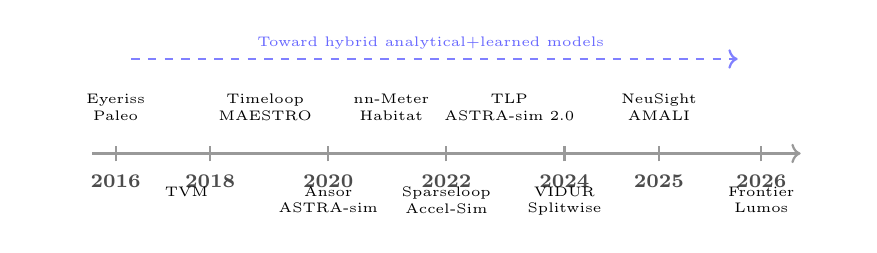
\begin{tikzpicture}[
    node distance=0.2cm,
    yearnode/.style={font=\scriptsize\bfseries, text=black!70},
    eventnode/.style={font=\tiny, text width=2cm, align=center},
    catnode/.style={font=\tiny, text=white, rounded corners=1pt, inner sep=2pt}
]
% Timeline base
\draw[thick, ->, black!40] (0,0) -- (9,0);
% Year markers
\foreach \x/\year in {0.3/2016, 1.5/2018, 3/2020, 4.5/2022, 6/2024, 7.2/2025, 8.5/2026} {
    \draw[thick, black!40] (\x,-0.1) -- (\x,0.1);
    \node[yearnode, below] at (\x,-0.15) {\year};
}
% Events
\node[eventnode, above] at (0.3,0.3) {Eyeriss\\Paleo};
\node[eventnode, below] at (1.2,-0.3) {TVM};
\node[eventnode, above] at (2.2,0.3) {Timeloop\\MAESTRO};
\node[eventnode, below] at (3,-0.3) {Ansor\\ASTRA-sim};
\node[eventnode, above] at (3.8,0.3) {nn-Meter\\Habitat};
\node[eventnode, below] at (4.5,-0.3) {Sparseloop\\Accel-Sim};
\node[eventnode, above] at (5.3,0.3) {TLP\\ASTRA-sim 2.0};
\node[eventnode, below] at (6,-0.3) {VIDUR\\Splitwise};
\node[eventnode, above] at (7.2,0.3) {NeuSight\\AMALI};
\node[eventnode, below] at (8.5,-0.3) {Frontier\\Lumos};
% Trend
\draw[thick, ->, blue!50, dashed] (0.5,1.2) -- (8.2,1.2);
\node[font=\tiny, text=blue!60, above] at (4.3,1.2) {Toward hybrid analytical+learned models};
\end{tikzpicture}%
}
\caption{Evolution of performance modeling tools (2016--2026). Early analytical frameworks gave way to systematic accelerator modeling and distributed training simulation. Recent work targets LLM-specific and hybrid approaches.}
\label{fig:timeline}
\end{figure}

% ==============================================================================
% SURVEY METHODOLOGY
% ==============================================================================
\section{Survey Methodology}
\label{sec:methodology}

We searched ACM Digital Library, IEEE Xplore, Semantic Scholar, and arXiv using terms related to ML performance modeling, with backward/forward citation tracking from seminal works.
Target venues include architecture (MICRO, ISCA, HPCA, ASPLOS), systems (MLSys, OSDI, SOSP, NSDI), and related (NeurIPS, MobiSys, DAC, ISPASS).
Papers must propose or evaluate a tool for predicting ML workload performance with quantitative evaluation; we exclude non-performance tasks and general-purpose workloads.
From 287 initial candidates, title/abstract screening yielded 118 papers; full-text review reduced the set to 53 that met all criteria, supplemented by 12 foundational works for context.
We cover 2016--2026 and classify each paper by \emph{methodology type} (analytical, simulation, trace-driven, ML-augmented, hybrid), \emph{target platform}, and \emph{abstraction level} (kernel, model, system).

\textbf{Related surveys and scope boundaries.}
Prior surveys address adjacent topics: Rakhshanfar and Zarandi~\cite{rakhshanfar2021survey} survey ML for processor DSE; Sze et al.~\cite{sze2017efficient} treat DNN hardware design (the foundation for Timeloop/MAESTRO); simulators such as GPGPU-Sim~\cite{gpgpusim2009}, gem5~\cite{binkert2011gem5}, and SST~\cite{sst2012} have been extensively used as validation targets in the performance modeling literature; and MLPerf~\cite{mlperf_training2020,mlperf_inference2020} standardizes \emph{measurement} rather than \emph{prediction}.
Early ML accelerator modeling (2014--2018) established foundational approaches: DianNao~\cite{diannao2014} introduced analytical dataflow modeling for dedicated accelerators, Eyeriss~\cite{eyeriss2016} systematized row-stationary dataflow analysis, and Paleo~\cite{paleo2017} pioneered layer-wise analytical estimation.
The closest prior work, Dudziak et al.~\cite{latencypredictorsnas2024}, compares edge device predictors for NAS; we broaden to the full landscape.

\textbf{Proprietary and vendor tools.}
NVIDIA's Nsight Compute~\cite{nsightcompute2019} and Nsight Systems are the most widely-used GPU profiling tools in practice; Google's internal TPU models underpin production scheduling but are undocumented.
We exclude these from evaluation as they cannot be independently reproduced, though surveyed tools frequently validate against Nsight Compute data.

\textbf{Compiler cost models and capacity planning.}
Beyond TVM/Ansor/TLP, relevant compiler models include Halide's autoscheduler~\cite{halide2013} (pioneered learned cost models), MLIR-based cost models~\cite{mlir2020}, and Triton's~\cite{triton2019} heuristic GPU kernel cost model.
At the system level, Pollux~\cite{pollux2021} and Sia~\cite{sia2023} use performance models for cluster scheduling and capacity planning---a distinct use case (optimizing workload placement) that shares modeling techniques with our surveyed tools.

This survey differs from all prior work by spanning the full methodology spectrum across all major platforms with reproducibility evaluation.

% ==============================================================================
% BACKGROUND
% ==============================================================================
\section{Background}
\label{sec:background}

\subsection{ML Workload Characteristics}
\label{subsec:workload-characteristics}

ML workloads are expressed as computation graphs whose operator shapes are statically known and amenable to analytical modeling. Frameworks such as PyTorch~\cite{pytorch2019} and TensorFlow~\cite{tensorflow2016} compile these graphs for execution, though MoE and dynamic inference introduce input-dependent control flow.
Performance depends on tensor-to-memory mapping (dataflow, tiling), KV cache management for LLM inference~\cite{vllm2023}, and at scale, compute--memory--network interactions across data, tensor, pipeline, and expert parallelism~\cite{llama3scaling2025}.
LLM inference splits into compute-bound prefill and memory-bound decode phases~\cite{splitwise2024}, both modeled under batched serving~\cite{sarathi2024,orca2022}.
Foundation model training introduces additional modeling challenges: long-context attention with quadratic memory scaling, activation checkpointing that trades compute for memory, and mixed-precision training where numerical format affects both speed and convergence~\cite{llama3scaling2025}.

\subsection{Modeling Methodologies}
\label{subsec:modeling-methodologies}

We classify approaches into five categories.
\textbf{Analytical models} express performance as closed-form functions (e.g., the roofline model~\cite{williams2009roofline}), offering microsecond evaluation but requiring per-architecture derivation.
\textbf{Cycle-accurate simulators} (GPGPU-Sim~\cite{gpgpusim2009}, Accel-Sim~\cite{accelsim2020}) achieve high fidelity at $1000$--$10000\times$ slowdown, serving primarily as validation oracles for the high-level methods that are the focus of this survey.
\textbf{Trace-driven simulators} (ASTRA-sim~\cite{astrasim2023}, VIDUR~\cite{vidur2024}) trade fidelity for orders-of-magnitude speedup.
\textbf{ML-augmented approaches} learn from profiling data (nn-Meter~\cite{nnmeter2021}) but may not generalize beyond training distributions.
\textbf{Hybrid approaches} combine analytical structure with learned components (NeuSight~\cite{neusight2025}, Habitat~\cite{habitat2021}), aiming to balance accuracy, speed, and interpretability.
Accuracy metrics---MAPE, RMSE, and rank correlation---vary across the literature, limiting direct comparison (Section~\ref{sec:eval-results}); ground-truth relies on hardware counters (PAPI~\cite{papi2000}, LIKWID~\cite{likwid2010}) or vendor profilers~\cite{nsightcompute2019}.

% ==============================================================================
% TAXONOMY
% ==============================================================================
\section{Taxonomy}
\label{sec:taxonomy}

We organize the literature along three dimensions.
The \emph{primary axis} is methodology type---how a tool predicts performance---because methodology determines the fundamental trade-offs between accuracy, speed, interpretability, and data requirements.
The \emph{secondary axes} are target platform and abstraction level, which together determine the scope and applicability of each tool.
We additionally characterize tools by workload coverage, identifying a temporal validation lag: tools published during the CNN era naturally validated on CNN workloads, while post-2023 tools increasingly target transformers and LLMs.

Table~\ref{tab:taxonomy-matrix} provides a unified view combining the coverage matrix (number of surveyed tools per methodology--platform cell) with trade-off profiles, with empty cells highlighting research gaps.
The dominant pairings are: analytical models for accelerators, cycle-accurate simulation for GPUs/CPUs, trace-driven simulation for distributed systems, and ML-augmented approaches for edge devices.

% --- Unified Taxonomy Table (merged from Tables 1+2, issue #192) ---
\begin{table*}[t]
\centering
\caption{Methodology taxonomy: coverage matrix and trade-off profile.
Platform columns show the number of surveyed tools per cell; \textbf{0} indicates an explicit research gap.
Speed, data requirements, and interpretability determine practical applicability; the failure mode column identifies the primary condition under which each methodology breaks down.}
\label{tab:taxonomy-matrix}
\small
\begin{tabular}{l|ccccc|cccc}
\toprule
 & \textbf{DNN} & & \textbf{Distrib.} & \textbf{Edge/} & & \textbf{Eval.} & \textbf{Data} & & \textbf{Failure} \\
\textbf{Methodology} & \textbf{Accel.} & \textbf{GPU} & \textbf{Systems} & \textbf{Mobile} & \textbf{CPU} & \textbf{Speed} & \textbf{Req.} & \textbf{Interp.} & \textbf{Mode} \\
\midrule
Analytical       & 3 & 3 & 2 & \textbf{0} & \textbf{0} & $\mu$s & None & High & Dynamic effects \\
Cycle-Accurate   & 1 & 2 & \textbf{0} & \textbf{0} & 1 & Hours & Binary & High & Scale \\
Trace-Driven     & \textbf{0} & \textbf{0} & 7 & \textbf{0} & \textbf{0} & Min. & Traces & Med. & Trace fidelity \\
ML-Augmented     & \textbf{0} & 3 & \textbf{0} & 3 & 1 & ms & Profiling & Low & Distrib.\ shift \\
Hybrid           & 1 & 2 & \textbf{0} & \textbf{0} & 1 & ms & Mixed & Med. & Training domain \\
\bottomrule
\end{tabular}
\end{table*}

Table~\ref{tab:taxonomy-matrix} reveals three structural gaps: (1)~trace-driven \emph{execution replay} simulation (as distinct from instruction-trace-driven cycle-accurate simulation such as Accel-Sim) is used exclusively for distributed systems; (2)~edge devices are served only by ML-augmented approaches, lacking hybrid alternatives; (3)~no ML-augmented tool targets distributed systems directly.
Methodologies cluster into two speed regimes: sub-millisecond (analytical, ML-augmented, hybrid) for DSE, and minutes-to-hours (simulation, trace-driven) for validation.

Figure~\ref{fig:tool-architecture} illustrates how tools from different methodology types compose: analytical engines provide fast base estimates, ML components learn residual corrections, and trace-driven simulators orchestrate system-level execution.

\begin{figure}[t]
\centering
\resizebox{\columnwidth}{!}{%
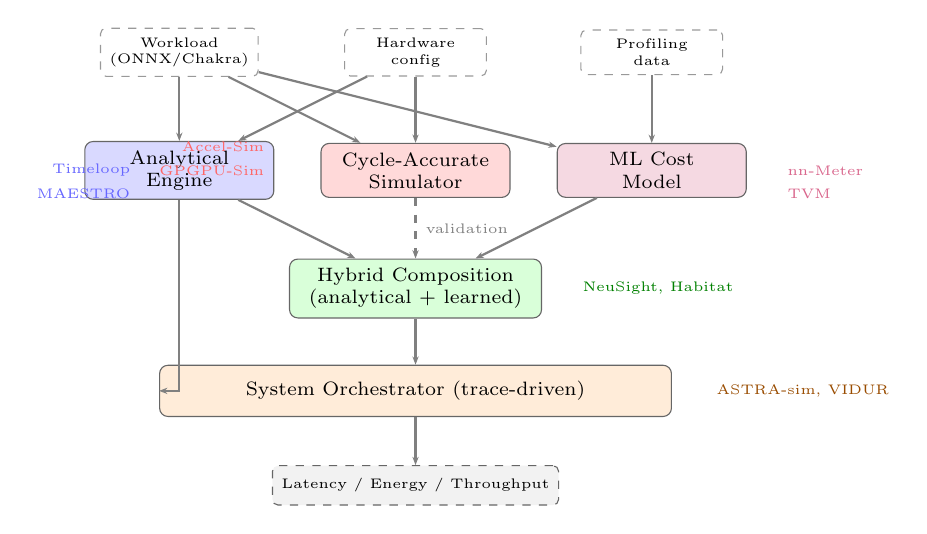
\begin{tikzpicture}[
    comp/.style={draw=black!60, rounded corners=3pt, minimum width=2.4cm, minimum height=0.65cm, align=center, font=\scriptsize},
    input/.style={draw=black!40, dashed, rounded corners=2pt, minimum width=1.8cm, minimum height=0.5cm, align=center, font=\tiny},
    arr/.style={-{Stealth[length=3pt]}, thick, black!50},
    lbl/.style={font=\tiny, text=black!50},
]

% Input layer
\node[input] (wl) at (0,4) {Workload\\(ONNX/Chakra)};
\node[input] (hw) at (3,4) {Hardware\\config};
\node[input] (prof) at (6,4) {Profiling\\data};

% Methodology layer
\node[comp, fill=blue!15] (analytical) at (0,2.5) {Analytical\\Engine};
\node[comp, fill=red!15] (simulator) at (3,2.5) {Cycle-Accurate\\Simulator};
\node[comp, fill=purple!15] (mlmodel) at (6,2.5) {ML Cost\\Model};

% Hybrid composition
\node[comp, fill=green!15, minimum width=3.2cm] (hybrid) at (3,1) {Hybrid Composition\\(analytical + learned)};

% System orchestration
\node[comp, fill=orange!15, minimum width=6.5cm] (system) at (3,-0.3) {System Orchestrator (trace-driven)};

% Output
\node[input, draw=black!60, fill=gray!10] (output) at (3,-1.5) {Latency / Energy / Throughput};

% Arrows - inputs to methods
\draw[arr] (wl) -- (analytical);
\draw[arr] (hw) -- (analytical);
\draw[arr] (hw) -- (simulator);
\draw[arr] (wl) -- (simulator);
\draw[arr] (prof) -- (mlmodel);
\draw[arr] (wl) -- (mlmodel);

% Arrows - methods to hybrid
\draw[arr] (analytical) -- (hybrid);
\draw[arr] (mlmodel) -- (hybrid);
\draw[arr, dashed, gray] (simulator) -- node[lbl, right] {validation} (hybrid);

% Arrows - to system
\draw[arr] (hybrid) -- (system);
\draw[arr] (analytical) |- (system);

% Arrows - output
\draw[arr] (system) -- (output);

% Example tools
\node[font=\tiny, text=blue!60, anchor=east] at (-0.5,2.5) {Timeloop};
\node[font=\tiny, text=blue!60, anchor=east] at (-0.5,2.2) {MAESTRO};
\node[font=\tiny, text=red!60, anchor=east] at (1.2,2.8) {Accel-Sim};
\node[font=\tiny, text=red!60, anchor=east] at (1.2,2.5) {GPGPU-Sim};
\node[font=\tiny, text=purple!60, anchor=west] at (7.6,2.5) {nn-Meter};
\node[font=\tiny, text=purple!60, anchor=west] at (7.6,2.2) {TVM};
\node[font=\tiny, text=green!50!black, anchor=west] at (5,1) {NeuSight, Habitat};
\node[font=\tiny, text=orange!60!black, anchor=west] at (6.7,-0.3) {ASTRA-sim, VIDUR};

\end{tikzpicture}%
}
\caption{Unified architecture showing how tool methodologies compose. Analytical engines and ML cost models feed into hybrid approaches, while system-level orchestrators (trace-driven) assemble component predictions into end-to-end estimates. Cycle-accurate simulators primarily serve as validation oracles.}
\label{fig:tool-architecture}
\end{figure}

\subsection{Methodology--Platform Pairings}
\label{subsec:by-methodology}

Table~\ref{tab:taxonomy-matrix} summarizes methodology trade-offs; Section~\ref{sec:survey} details individual tools.
Platform constrains methodology: \textbf{accelerators} use analytical models (Timeloop~\cite{timeloop2019}, MAESTRO~\cite{maestro2019}); \textbf{GPUs} span all five types; \textbf{distributed systems} require trace-driven simulation (ASTRA-sim~\cite{astrasim2023}, VIDUR~\cite{vidur2024}); \textbf{edge devices} rely on ML-augmented approaches (nn-Meter~\cite{nnmeter2021}, LitePred~\cite{litepred2024}); \textbf{CPUs}~\cite{concorde2025,granite2022} are least studied.
Abstraction level determines composition errors (Figure~\ref{fig:abstraction-levels}): kernel-level tools achieve 2--3\% error, model-level 5--12\%, and system-level 5--15\%, with errors propagating through the chain---a gap we quantify in Section~\ref{sec:eval-framework}.

\begin{figure}[t]
\centering
\resizebox{\columnwidth}{!}{%
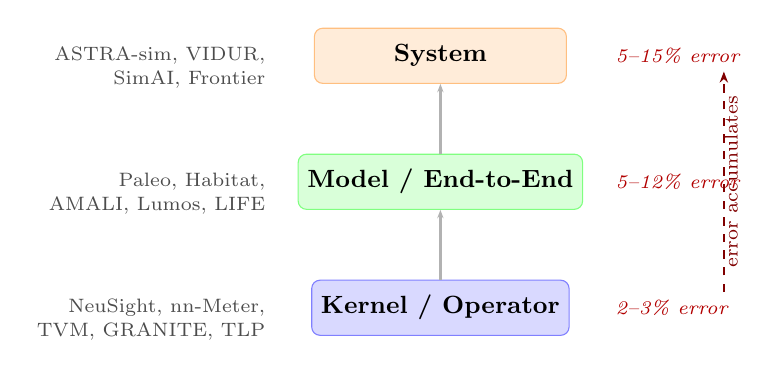
\begin{tikzpicture}[
  level/.style={draw, rounded corners=3pt, minimum width=3.2cm, minimum height=0.7cm, align=center, font=\small\bfseries},
  tool/.style={font=\scriptsize, text=black!70},
  err/.style={font=\scriptsize\itshape, text=red!70!black},
  arrow/.style={-{Stealth[length=3pt]}, thick, gray!60},
  compos/.style={-{Stealth[length=4pt]}, thick, red!50!black, dashed},
]

% Levels (bottom to top)
\node[level, fill=blue!15, draw=blue!50] (kernel) at (0,0) {Kernel / Operator};
\node[level, fill=green!15, draw=green!50] (model) at (0,1.6) {Model / End-to-End};
\node[level, fill=orange!15, draw=orange!50] (system) at (0,3.2) {System};

% Composition arrows between levels
\draw[arrow] (kernel) -- (model);
\draw[arrow] (model) -- (system);

% Tool names (left side)
\node[tool, anchor=east] at (-2.1,0) {NeuSight, nn-Meter,};
\node[tool, anchor=east] at (-2.1,-0.3) {TVM, GRANITE, TLP};
\node[tool, anchor=east] at (-2.1,1.6) {Paleo, Habitat,};
\node[tool, anchor=east] at (-2.1,1.3) {AMALI, Lumos, LIFE};
\node[tool, anchor=east] at (-2.1,3.2) {ASTRA-sim, VIDUR,};
\node[tool, anchor=east] at (-2.1,2.9) {SimAI, Frontier};

% Error ranges (right side)
\node[err, anchor=west] at (2.1,0) {2--3\% error};
\node[err, anchor=west] at (2.1,1.6) {5--12\% error};
\node[err, anchor=west] at (2.1,3.2) {5--15\% error};

% Composition problem annotation
\draw[compos] (3.6,0.2) -- (3.6,3.0);
\node[font=\scriptsize, text=red!50!black, rotate=90, anchor=south] at (3.9,1.6) {error accumulates};

\end{tikzpicture}%
}
\caption{Abstraction level hierarchy and the composition problem. Tools operate at one of three levels; composing predictions across levels accumulates error. Error ranges are representative values from surveyed papers.}
\label{fig:abstraction-levels}
\end{figure}

\subsection{Workload Coverage and Validation Gaps}
\label{subsec:workload-coverage}

Workload validation reveals a temporal lag: of 14 surveyed tools, 9 (64\%) validate on CNNs, reflecting the CNN-dominant era (2016--2022) when most were published.
The lag is closing---post-2023 tools (VIDUR, Frontier, Lumos, SimAI) validate exclusively on transformers/LLMs---but \textbf{no surveyed tool has been validated on diffusion models or dynamic inference workloads}~\cite{dynamicreasoning2026}, only Frontier~\cite{frontier2025} validates MoE, and no tool offers validated transformer prediction across the full kernel-to-system stack.
Section~\ref{sec:eval-results} provides our independent assessment of these claimed capabilities.

% ==============================================================================
% SURVEY OF APPROACHES
% ==============================================================================
\section{Survey of Approaches}
\label{sec:survey}

This section surveys performance modeling tools for ML workloads, organized by target platform, examining modeling challenges, available tools, and their strengths and limitations.
Table~\ref{tab:survey-summary} provides a comprehensive comparison.

\begin{table*}[t]
\centering
\caption{Summary of surveyed performance modeling tools for ML workloads, organized by target platform. \textbf{Methodology}: A=Analytical, S=Simulation, T=Trace-driven, M=ML-augmented, H=Hybrid. $^*$Accuracy measures surrogate-vs-simulator fidelity, not real hardware error. $^\dagger$Reported accuracy unverifiable due to reproducibility issues. $^\ddagger$No accuracy baseline against real hardware reported.}
\label{tab:survey-summary}
\small
\begin{tabular}{lllllll}
\toprule
\textbf{Tool} & \textbf{Platform} & \textbf{Method} & \textbf{Target} & \textbf{Accuracy} & \textbf{Speed} & \textbf{Key Capability} \\
\midrule
\multicolumn{7}{l}{\textit{DNN Accelerator Modeling}} \\
Timeloop~\cite{timeloop2019} & NPU & A & Latency/Energy & 5--10\% & $\mu$s & Loop-nest DSE \\
MAESTRO~\cite{maestro2019} & NPU & A & Latency/Energy & 5--15\% & $\mu$s & Data-centric directives \\
Sparseloop~\cite{sparseloop2022} & NPU & A & Sparse tensors & 5--10\% & $\mu$s & Compression modeling \\
PyTorchSim~\cite{pytorchsim2025} & NPU & S & Cycle-accurate & N/A$^\ddagger$ & Hours & PyTorch 2 integration \\
ArchGym~\cite{archgym2023} & Multi & H & Multi-objective & 0.61\%$^*$ & ms & ML-aided DSE \\
\midrule
\multicolumn{7}{l}{\textit{GPU Performance Modeling}} \\
Accel-Sim~\cite{accelsim2020} & GPU & S & Cycle-accurate & 10--20\% & Hours & SASS trace-driven \\
GPGPU-Sim~\cite{gpgpusim2009} & GPU & S & Cycle-accurate & 10--20\% & Hours & CUDA workloads \\
AMALI~\cite{amali2025} & GPU & A & LLM inference & 23.6\% & ms & Memory hierarchy \\
NeuSight~\cite{neusight2025} & GPU & H & Kernel/E2E latency & 2.3\% & ms & Tile-based prediction \\
Habitat~\cite{habitat2021} & GPU & H & Training time & 11.8\% & Per-kernel & Wave scaling \\
\midrule
\multicolumn{7}{l}{\textit{Distributed Training and LLM Serving}} \\
ASTRA-sim~\cite{astrasim2023} & Distributed & T & Training time & 5--15\% & Minutes & Collective modeling \\
SimAI~\cite{simai2025} & Distributed & T & Training time & 1.9\% & Minutes & Full-stack simulation \\
Lumos~\cite{lumos2025} & Distributed & T & LLM training & 3.3\% & Minutes & H100 training \\
VIDUR~\cite{vidur2024} & GPU cluster & T & LLM serving & $<$5\% & Seconds & Prefill/decode phases \\
Frontier~\cite{frontier2025} & Distributed & T & MoE inference & --- & Minutes & Stage-centric sim. \\
TrioSim~\cite{triosim2025} & Multi-GPU & T & DNN training & N/A$^\ddagger$ & Minutes & Lightweight multi-GPU \\
\midrule
\multicolumn{7}{l}{\textit{Edge Device Modeling}} \\
nn-Meter~\cite{nnmeter2021} & Edge & M & Latency & $<$1\%$^\dagger$ & ms & Kernel detection \\
LitePred~\cite{litepred2024} & Edge & M & Latency & 0.7\% & ms & 85-platform transfer \\
HELP~\cite{help2021} & Multi & M & Latency & 1.9\% & ms & 10-sample adaptation \\
\midrule
\multicolumn{7}{l}{\textit{Compiler Cost Models}} \\
TVM~\cite{tvm2018} & GPU & M & Schedule perf. & $\sim$15\% & ms & Autotuning guidance \\
Ansor~\cite{ansor2020} & GPU & M & Schedule perf. & $\sim$15\% & ms & Program sampling \\
TLP~\cite{tlp2023} & GPU & M & Tensor program & $<$10\% & ms & Transformer cost model \\
\bottomrule
\end{tabular}
\end{table*}

\subsection{DNN Accelerator Modeling}
\label{subsec:accelerator-modeling}

The analytical tractability of DNN accelerator modeling stems from the regularity of computation~\cite{sze2017efficient}, building on early characterization by DianNao~\cite{diannao2014} and Eyeriss~\cite{eyeriss2016}.
Timeloop~\cite{timeloop2019} enumerates mappings of convolution loop nests to a spatial-temporal hardware hierarchy, finding optimal dataflow in microseconds (5--10\% error, $2000\times$ speedup) via capacity-based pruning.
MAESTRO~\cite{maestro2019} uses a compact ``data-centric'' representation, trading enumeration completeness for specification simplicity.
Sparseloop~\cite{sparseloop2022} extends to sparse tensors with format-specific access models (CSR, bitmap); SCALE-Sim~\cite{scalesim2019} provides cycle-accurate systolic array simulation for validation.
PyTorchSim~\cite{pytorchsim2025} and ArchGym~\cite{archgym2023} (0.61\% RMSE vs.\ simulator, not hardware) represent newer integration approaches.
This is the most mature subdomain; emerging PIM tools~\cite{upimulator2024,attacc2024,neupims2024,paise2025} also lack hardware validation.

\subsection{GPU Performance Modeling}
\label{subsec:gpu-modeling}

GPGPU-Sim~\cite{gpgpusim2009} and Accel-Sim~\cite{accelsim2020} achieve 0.90--0.97 IPC correlation at $1000$--$10000\times$ slowdown, integrating with memory models (DRAMSim3~\cite{dramsim3_2020}, Ramulator~2.0~\cite{ramulator2_2023}) for DRAM timing~\cite{dramsim2_2011,ramulator2015}; reverse-engineering~\cite{dissectinggpu2025} improved Accel-Sim to 13.98\% MAPE.
NeuSight~\cite{neusight2025} achieves 2.3\% MAPE by decomposing kernels into \emph{tiles} matching CUDA thread blocks---this succeeds because each SM's execution depends on locally measurable arithmetic intensity, shared memory, and register pressure.
AMALI~\cite{amali2025} averages data movement over entire kernels, losing per-SM occupancy information (23.6\% MAPE); the roofline model~\cite{williams2009roofline,rooflinellm2024} provides upper bounds.
Habitat~\cite{habitat2021} achieves 11.8\% cross-GPU transfer via wave scaling.
VIDUR~\cite{vidur2024} simulates LLM serving at $<$5\% error; TVM~\cite{tvm2018}/Ansor~\cite{ansor2020} ($\sim$15\%), TLP~\cite{tlp2023} ($<$10\%), and recent tools~\cite{life2025,hermes2025,omniwise2025,swizzleperf2025,synperf2025} target inference and autotuning~\cite{tenset2021}.

\subsection{Distributed Training and LLM Serving}
\label{subsec:distributed-modeling}

Distributed systems require modeling communication, synchronization, and parallelism strategies~\cite{megatronlm2020,gpipe2019,zero2020}.
The speed--fidelity hierarchy reflects modeling granularity: VIDUR models serving at the \emph{request level} (seconds); ASTRA-sim~\cite{astrasim2023} replays Chakra traces~\cite{chakra2023} at the \emph{collective level} (5--15\%); SimAI~\cite{simai2025} models \emph{NCCL-level} chunk reductions (1.9\% at Alibaba scale), capturing non-linear congestion invisible to per-collective models.
Echo~\cite{echo2024} scales to 10K+ devices; Lumos~\cite{lumos2025} achieves 3.3\% on H100s; PRISM~\cite{prism2025} provides prediction intervals.
Paleo~\cite{paleo2017} pioneered analytical estimation; MAD Max~\cite{madmax2024} and Sailor~\cite{sailor2025} extend it.
For inference serving, DistServe~\cite{distserve2024}, Frontier~\cite{frontier2025} (MoE), POD-Attention~\cite{podattention2025}, AQUA~\cite{aqua2025}, and ThrottLL'eM~\cite{throttllem2025} address scheduling, disaggregation, and power; speculative decoding~\cite{medusa2024} creates a moving target.

\subsection{Edge Device Modeling}
\label{subsec:edge-modeling}

nn-Meter~\cite{nnmeter2021} claims $<$1\% MAPE but is unverifiable due to dependency failures (Section~\ref{sec:eval-results}); LitePred~\cite{litepred2024} achieves 0.7\% across 85 platforms; HELP~\cite{help2021} reaches 1.9\% with 10-sample meta-learning.
ESM~\cite{esm2025} finds well-tuned random forests match deep learning surrogates, and transfer learning provides 22.5\% improvement~\cite{latencypredictorsnas2024}---suggesting data quality matters more than model sophistication.

% ==============================================================================
% EVALUATION FRAMEWORK
% ==============================================================================
\section{Evaluation Framework}
\label{sec:eval-framework}

Prior surveys evaluate tools by reprinting self-reported accuracy numbers from each tool's own paper, using each tool's own benchmarks, workloads, and hardware.
This makes cross-tool comparison methodologically unsound: a tool reporting 2\% MAPE on GPU kernels is solving a fundamentally different problem than one reporting 5\% on distributed training.
We propose the \textbf{Multi-dimensional Tool Assessment Protocol (MTAP)}, a principled evaluation framework that (1)~defines comparable evaluation dimensions beyond accuracy, (2)~measures compositional fidelity---how kernel-level predictions degrade when composed into system-level estimates---and (3)~assesses practical deployment viability over time.
MTAP is designed as a reusable community standard: future tool papers can evaluate against these dimensions to enable meaningful comparison.

\textbf{Relationship to existing evaluation approaches.}
Multi-dimensional evaluation is established practice in adjacent domains: MLPerf~\cite{mlperf_training2020,mlperf_inference2020} standardizes throughput, latency, and power for ML \emph{measurement}; SPEC and TPC define reproducible protocols for system and database benchmarking; artifact evaluation committees at MICRO and ISCA assess deployment viability and reproducibility.
However, none of these frameworks address performance \emph{prediction}---where the central question is not ``how fast does the workload run?'' but ``how accurately can a tool predict how fast it \emph{will} run, on hardware not yet available?''
Prediction introduces challenges absent from measurement: compositional error propagation across abstraction levels, generalization to unseen hardware, and temporal stability as software stacks evolve.
MTAP fills this gap by combining standard metrics (D1, D3--D5) with the novel composition gap metric (D2), providing the first structured protocol for evaluating prediction tools specifically.
The closest prior work, Dudziak et al.~\cite{latencypredictorsnas2024}, compares edge predictors on D1 and D3 metrics but omits D2, D4, and D5.

\textbf{Formal scoring.}
Each tool $t$ receives a composite MTAP score $S(t) = \sum_{i=1}^{5} w_i \cdot d_i(t)$, where $w = (0.4, 0.2, 0.2, 0.1, 0.1)$ are dimension weights and each $d_i(t) \in \{0, 1, 2, 3\}$ maps to \{Fail, Low, Medium, High\} via the rubrics in Table~\ref{tab:scoring-rubrics}.
Weights reflect practitioner priorities: prediction fidelity dominates because incorrect predictions lead to flawed design decisions; compositional and generalization fidelity share equal weight as they determine whether a tool can be used beyond its original evaluation context; deployment viability and extensibility receive lower weight as they affect adoption friction rather than correctness.
To verify that findings are robust to weight choice, we conduct a sensitivity analysis: under uniform weights $w_{\text{uni}} = (0.2, 0.2, 0.2, 0.2, 0.2)$ and deployment-heavy weights $w_{\text{dep}} = (0.2, 0.2, 0.1, 0.3, 0.2)$, the ordinal tool ranking remains unchanged---VIDUR, ASTRA-sim, and Timeloop score within 0.2 points of each other under all three schemes, while nn-Meter scores $\leq 0.4$ under every scheme (Section~\ref{subsec:cross-cutting-findings}).

\textbf{Scoring rubrics.}
Table~\ref{tab:scoring-rubrics} defines explicit thresholds for each dimension, ensuring that two independent evaluators applying MTAP to the same tool would assign the same scores.
For D1, scoring depends on whether accuracy is independently verified or self-reported; for D2--D5, criteria are binary or threshold-based.

\begin{table}[t]
\centering
\caption{MTAP scoring rubrics. Each dimension maps measurable criteria to ordinal scores. D1 thresholds apply within a tool's problem domain; cross-domain comparison is not meaningful.}
\label{tab:scoring-rubrics}
\small
\begin{tabular}{lp{5.2cm}}
\toprule
\textbf{Score} & \textbf{D1: Prediction Fidelity} \\
\midrule
H (3) & MAPE $<$ 5\% AND hardware-validated AND $\rho_s > 0.95$ \\
M (2) & MAPE $<$ 15\% OR self-reported $<$ 5\% without independent verification \\
L (1) & MAPE $<$ 25\% OR limited workload validation \\
F (0) & No working prediction OR MAPE $>$ 25\% \\
\midrule
 & \textbf{D2: Compositional Fidelity} \\
\midrule
H (3) & Validated multi-level composition with $\gamma < 0.10$ \\
M (2) & Single-level prediction with documented scope \\
L (1) & Composition attempted but $\gamma > 0.20$ \\
F (0) & No composition capability or undocumented scope \\
\midrule
 & \textbf{D3: Generalization Robustness} \\
\midrule
H (3) & Cross-workload AND cross-hardware transfer validated \\
M (2) & One of workload or hardware transfer validated \\
L (1) & Single-workload or single-hardware only \\
F (0) & Tool fails on workloads outside training set \\
\midrule
 & \textbf{D4: Deployment Viability} \\
\midrule
H (3) & Docker-based, $<$30\,min to first prediction, CI-tested \\
M (2) & Builds with manual setup, $<$2\,hr to first prediction \\
L (1) & Requires significant patching, $>$2\,hr setup \\
F (0) & Complete build or runtime failure \\
\midrule
 & \textbf{D5: Extensibility} \\
\midrule
H (3) & Config-driven new hardware, standard workload formats \\
M (2) & New hardware via config but custom workload format \\
L (1) & Requires code changes for new hardware or workloads \\
F (0) & Closed-source or no extension mechanism \\
\bottomrule
\end{tabular}
\end{table}

\subsection{Evaluation Dimensions}
\label{subsec:eval-dimensions}

MTAP evaluates tools along five dimensions weighted by their importance for practitioner adoption (Figure~\ref{fig:mtap-framework}).

\begin{figure}[t]
\centering
\resizebox{\columnwidth}{!}{%
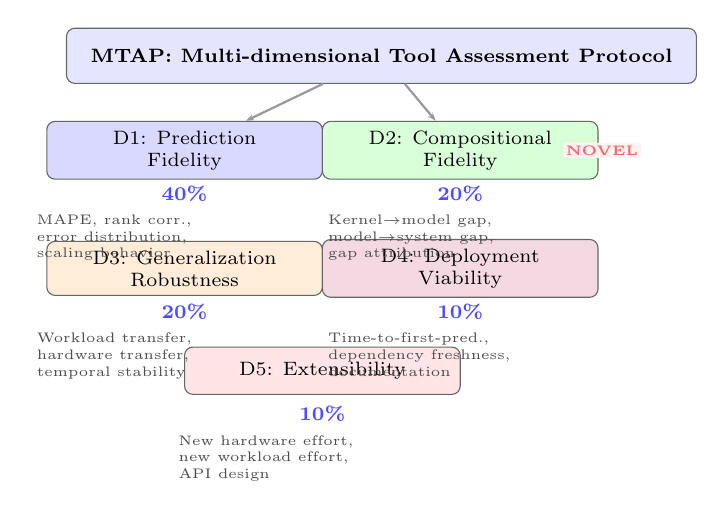
\begin{tikzpicture}[
    dim/.style={draw=black!60, rounded corners=3pt, minimum width=3.5cm, minimum height=0.6cm, align=center, font=\scriptsize},
    subdim/.style={font=\tiny, text=black!70, align=left},
    weight/.style={font=\scriptsize\bfseries, text=blue!70},
    arr/.style={-{Stealth[length=3pt]}, thick, black!40},
]

% Main framework box
\node[dim, fill=blue!10, minimum width=8cm, minimum height=0.7cm] (title) at (4,5.2) {\textbf{MTAP: Multi-dimensional Tool Assessment Protocol}};

% Dimensions
\node[dim, fill=blue!15] (d1) at (1.5,4) {D1: Prediction\\Fidelity};
\node[dim, fill=green!15] (d2) at (5,4) {D2: Compositional\\Fidelity};
\node[dim, fill=orange!15] (d3) at (1.5,2.5) {D3: Generalization\\Robustness};
\node[dim, fill=purple!15] (d4) at (5,2.5) {D4: Deployment\\Viability};
\node[dim, fill=red!10] (d5) at (3.25,1.2) {D5: Extensibility};

% Weights
\node[weight] at (1.5,3.45) {40\%};
\node[weight] at (5,3.45) {20\%};
\node[weight] at (1.5,1.95) {20\%};
\node[weight] at (5,1.95) {10\%};
\node[weight] at (3.25,0.65) {10\%};

% Subdimensions
\node[subdim, anchor=north west] at (-0.5,3.3) {MAPE, rank corr.,\\error distribution,\\scaling behavior};
\node[subdim, anchor=north west] at (3.2,3.3) {Kernel$\rightarrow$model gap,\\model$\rightarrow$system gap,\\gap attribution};
\node[subdim, anchor=north west] at (-0.5,1.8) {Workload transfer,\\hardware transfer,\\temporal stability};
\node[subdim, anchor=north west] at (3.2,1.8) {Time-to-first-pred.,\\dependency freshness,\\documentation};
\node[subdim, anchor=north west] at (1.3,0.5) {New hardware effort,\\new workload effort,\\API design};

% Arrows from title
\draw[arr] (title) -- (d1);
\draw[arr] (title) -- (d2);

% Novel marker
\node[font=\tiny\bfseries, text=red!60, fill=red!5, rounded corners=1pt, inner sep=1pt] at (6.8,4) {NOVEL};

\end{tikzpicture}%
}
\caption{The MTAP evaluation framework. Dimension weights reflect importance for practitioner adoption. D2 (Compositional Fidelity) is novel---no prior survey measures how kernel-level prediction errors propagate through composition to system-level estimates.}
\label{fig:mtap-framework}
\end{figure}

\textbf{D1: Prediction Fidelity (40\%).}
Beyond mean absolute percentage error (MAPE), we measure (a)~\emph{rank accuracy} via Spearman rank correlation---whether the tool correctly orders configurations matters more for DSE than absolute error; (b)~\emph{error distribution} rather than just mean error---a tool with 5\% MAPE but 30\% max error is worse for design than one with 8\% MAPE and 12\% max; (c)~\emph{scaling behavior}---how accuracy degrades as workload size, batch size, or device count increases.
Formally, for a workload set $W$ and hardware configuration $h$, the D1 score is a threshold function: $d_1(t) = \min\bigl(g_{\text{MAPE}}\bigl(\text{MAPE}(t,W,h)\bigr),\ g_{\rho}\bigl(\rho_s(t,W,h)\bigr)\bigr)$, where $g_{\text{MAPE}}$ and $g_{\rho}$ map to $\{0,1,2,3\}$ via the thresholds in Table~\ref{tab:scoring-rubrics}, $\rho_s$ is the Spearman rank correlation, and the minimum ensures that strong accuracy with poor rank ordering (or vice versa) does not receive a high score.
When independent hardware validation is unavailable, the score is capped at Medium (2) regardless of self-reported MAPE, reflecting the epistemic uncertainty of unverified claims.
Self-reported accuracy values are organized by problem domain; we do not rank tools across incomparable domains (Section~\ref{subsec:self-reported}).

\textbf{D2: Compositional Fidelity (20\%)---Novel.}
This dimension is unique to MTAP.
The composition problem (Figure~\ref{fig:error-composition}) is well-known qualitatively but has never been \emph{measured systematically}: kernel-level predictions (2--3\% error) must be composed into model-level (5--12\%) and system-level (5--15\%) estimates, with inter-kernel overheads (launch latency, memory allocation, synchronization) creating a gap that no tool explicitly bridges.
We define the \emph{composition gap ratio} $\gamma = |\hat{T}_{\text{model}} - \sum_k \hat{T}_k| / \sum_k \hat{T}_k$, where $\hat{T}_k$ are predicted kernel latencies and $\hat{T}_{\text{model}}$ is measured end-to-end latency; $\gamma > 0$ indicates unmodeled inter-kernel overhead.
We measure: (a)~kernel-to-model gap $\gamma_{\text{K}\to\text{M}}$; (b)~model-to-system gap $\gamma_{\text{M}\to\text{S}}$---single-device prediction vs.\ multi-device measured; (c)~gap attribution---decomposing $\gamma$ into kernel prediction error vs.\ inter-kernel overhead vs.\ communication modeling error.

\textbf{D3: Generalization Robustness (20\%).}
We assess: (a)~\emph{workload transfer}---do CNN-trained models generalize to transformers?; (b)~\emph{hardware transfer}---can GPU-A profiles predict GPU-B performance (Habitat's claimed capability)?; (c)~\emph{temporal stability}---does accuracy hold across software stack versions?
nn-Meter's complete failure due to scikit-learn version incompatibility (Section~\ref{subsec:per-tool-results}) demonstrates that temporal stability is a first-class concern.

\textbf{D4: Deployment Viability (10\%).}
Practical adoption depends on: (a)~\emph{time-to-first-prediction}---elapsed time from \texttt{git clone} to first valid output; (b)~\emph{deployment robustness}---Docker availability, dependency freshness, platform compatibility; (c)~\emph{documentation quality}---can a practitioner use the tool without contacting the original authors?
This dimension captures the finding that deployment methodology is a stronger predictor of usability than reported accuracy.

\textbf{D5: Extensibility (10\%).}
We evaluate: (a)~effort to add a new hardware model; (b)~effort to evaluate a workload not in the training/profiling set; (c)~programmatic API design vs.\ config-file-only interfaces.

\subsection{Experimental Design}
\label{subsec:experimental-design}

We apply MTAP using a systematic tools $\times$ workloads $\times$ metrics design (Table~\ref{tab:experiment-matrix}).
Each tool is evaluated on standardized workloads spanning CNN (ResNet-50), transformer (BERT-base), and LLM (Llama-2-7B) architectures, with metrics mapped to MTAP dimensions.
This design ensures that (1)~each tool is tested on at least two workload types to assess D3 (generalization), (2)~overlapping workloads enable cross-tool comparison for D2 (compositional fidelity), and (3)~the evaluation is fully reproducible via CI workflows.

\begin{table}[t]
\centering
\caption{MTAP experimental design matrix. Each cell indicates the MTAP dimension(s) assessed. Dashes indicate inapplicable tool--workload pairings.}
\label{tab:experiment-matrix}
\small
\begin{tabular}{lccc}
\toprule
 & \textbf{ResNet-50} & \textbf{BERT} & \textbf{Llama-2} \\
\textbf{Tool} & (Conv+FC) & (Attention) & (Serving) \\
\midrule
Timeloop & D1,D2 & --- & --- \\
ASTRA-sim & D1,D2,D3 & --- & --- \\
VIDUR & --- & --- & D1,D3,D4 \\
NeuSight & D1,D2 & D1,D3 & --- \\
nn-Meter & D1,D4 & D1,D3 & --- \\
\bottomrule
\end{tabular}
\end{table}

\textbf{Failure mode taxonomy.}
We classify tool evaluation failures into four categories to distinguish fundamental limitations from engineering issues:
\emph{(F1)~Build failure}---the tool cannot compile or install on the evaluation platform (nn-Meter's scikit-learn incompatibility);
\emph{(F2)~Runtime failure}---the tool builds but crashes or hangs on target workloads;
\emph{(F3)~Silent inaccuracy}---the tool produces output that disagrees with known baselines by $>$50\%, indicating a configuration or modeling error rather than expected prediction error;
\emph{(F4)~Scope mismatch}---the tool is applied outside its designed scope (e.g., using an accelerator-specific tool for GPU prediction).
Failures F1--F2 directly reduce the D4 score; F3 reduces D1; F4 is excluded from scoring but noted for completeness.

\subsection{Protocol and Reproducibility}
\label{subsec:eval-protocol}

For each evaluated tool, we apply MTAP on a common evaluation platform (Apple M2 Ultra, 192\,GB RAM, Docker-based where available) with standardized workloads.
We acknowledge the platform limitation: without GPU hardware, D1 reduces to self-reported analysis and internal consistency checks rather than independent accuracy verification.
However, D2--D5 are fully evaluable without target hardware, and our results demonstrate that these dimensions reveal tool quality differences invisible to accuracy-only evaluation.

\textbf{Statistical validation.}
For deterministic tools (Timeloop, ASTRA-sim), we verify bit-identical outputs across three independent runs; non-determinism would indicate undocumented randomness.
For stochastic tools (VIDUR with Poisson arrivals), we report mean and P99 latency across fixed random seeds and verify that inter-run variance is below 1\% of mean---confirming that seed control provides reproducible evaluation.

\textbf{Cross-tool comparison protocol.}
Where tool scopes overlap (e.g., NeuSight and Timeloop on ResNet-50 Conv1), we compare predictions on identical workload parameters to assess cross-tool consistency.
Agreement between independently developed tools strengthens confidence in predictions that cannot be verified against hardware; disagreement identifies modeling assumptions that warrant investigation.
We do not compare tools across different abstraction levels or problem domains, as such comparisons are methodologically unsound (Section~\ref{subsec:self-reported}).

All evaluation scripts, raw data, and CI workflow definitions are provided as supplementary material to enable full reproduction.

\subsection{Limitations of MTAP}
\label{subsec:mtap-limitations}

We identify four limitations of the current MTAP instantiation.
\emph{First}, D1 scoring without GPU hardware relies on self-reported accuracy and is capped at Medium; independent verification would strengthen these assessments.
\emph{Second}, D2 (Compositional Fidelity) is defined precisely ($\gamma$ ratio) but cannot be measured end-to-end with current tools---no tool provides validated kernel-to-system composition, making this dimension aspirational for the field rather than immediately measurable.
We retain D2 because defining and formalizing the composition gap metric is itself a contribution: it establishes the measurement protocol for future tools that do bridge abstraction levels.
\emph{Third}, $N=5$ evaluated tools is sufficient for case-study-level findings but too small for statistical generalization; findings should be interpreted as structured qualitative assessments rather than population statistics.
\emph{Fourth}, dimension weights ($w$) reflect our assessment of practitioner priorities; the sensitivity analysis in Section~\ref{subsec:cross-cutting-findings} shows that ordinal rankings are stable under reasonable weight perturbations, but alternative weighting schemes (e.g., deployment-first) would shift emphasis.

% ==============================================================================
% EVALUATION RESULTS
% ==============================================================================
\section{Evaluation Results}
\label{sec:eval-results}

We evaluate five tools spanning methodology types: Timeloop (analytical), ASTRA-sim (trace-driven, distributed), VIDUR (trace-driven, LLM serving), nn-Meter (ML-augmented, edge), and NeuSight (hybrid, GPU), applying MTAP across all five dimensions.
Table~\ref{tab:mtap-results} summarizes the multi-dimensional assessment.

\begin{table}[t]
\centering
\caption{MTAP multi-dimensional assessment of five tools. Scores: \textbf{H}=high (3), \textbf{M}=medium (2), \textbf{L}=low (1), \textbf{F}=fail (0), per rubrics in Table~\ref{tab:scoring-rubrics}. $S(t)$: composite score. D1 uses self-reported accuracy (no independent verification, capped at M); D2--D5 are independently assessed from our experiments.}
\label{tab:mtap-results}
\small
\begin{tabular}{lcccccc}
\toprule
 & \textbf{D1} & \textbf{D2} & \textbf{D3} & \textbf{D4} & \textbf{D5} & $\boldsymbol{S(t)}$ \\
\textbf{Tool} & \textbf{Fidelity} & \textbf{Comp.} & \textbf{Gen.} & \textbf{Deploy} & \textbf{Ext.} & \\
\midrule
VIDUR & M ($<$5\%) & H & L & H & M & 2.1 \\
Timeloop & M (5--10\%) & M & M & M & H & 2.1 \\
ASTRA-sim & M (5--15\%) & M & M & H & H & 2.2 \\
NeuSight & M (2.3\%) & M & L & L & L & 1.5 \\
nn-Meter & F ($<$1\%$^\dagger$) & F & F & F & F & 0.0 \\
\bottomrule
\end{tabular}
\end{table}

\subsection{D1: Self-Reported Accuracy Analysis}
\label{subsec:self-reported}

Self-reported accuracy values are \textbf{not comparable across problem domains}: each tool uses its own benchmarks, workloads, and hardware (Figure~\ref{fig:accuracy-speed}).
Within each domain, meaningful comparisons emerge.
\emph{Accelerator modeling} (5--15\% MAPE) is most analytically tractable---Timeloop (5--10\%) and MAESTRO (5--15\%) achieve tight bounds through loop-nest enumeration.
\emph{GPU kernel prediction} (2--12\%) spans a wider range: NeuSight (2.3\%) succeeds via tile-level decomposition; Habitat (11.8\%) trades accuracy for cross-GPU transfer.
\emph{Distributed systems} (2--15\%) exhibit the widest range, reflecting modeling granularity differences from request-level (VIDUR, $<$5\%) to NCCL-level (SimAI, 1.9\%).
\emph{Edge prediction} (0.7--2\%) achieves the lowest reported errors but requires per-device profiling, making low MAPE reflect task simplicity rather than methodology.

\begin{figure}[t]
\centering
\resizebox{\columnwidth}{!}{%
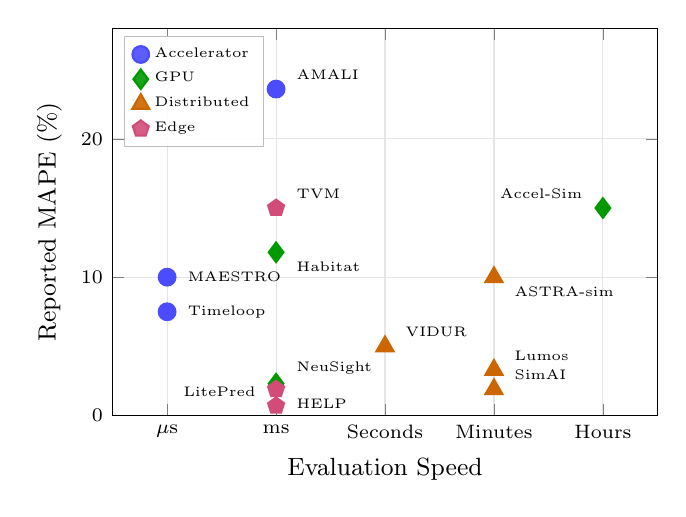
\begin{tikzpicture}
\begin{axis}[
    xlabel={Evaluation Speed},
    ylabel={Reported MAPE (\%)},
    ymin=0, ymax=28,
    xmin=-0.5, xmax=4.5,
    xtick={0,1,2,3,4},
    xticklabels={$\mu$s, ms, Seconds, Minutes, Hours},
    xticklabel style={font=\scriptsize},
    yticklabel style={font=\scriptsize},
    xlabel style={font=\small},
    ylabel style={font=\small},
    height=6.5cm,
    width=8.5cm,
    grid=both,
    grid style={gray!20},
    legend style={at={(0.02,0.98)}, anchor=north west, font=\tiny, draw=gray!50, fill=white, fill opacity=0.9, text opacity=1},
    legend cell align={left},
]
% Accelerator domain (blue)
\addplot[only marks, mark=*, mark size=3pt, blue!70, thick] coordinates {(0,7.5) (0,10) (1,23.6)};
% GPU domain (green)
\addplot[only marks, mark=diamond*, mark size=3.5pt, green!60!black, thick] coordinates {(1,2.3) (1,11.8) (4,15)};
% Distributed domain (orange)
\addplot[only marks, mark=triangle*, mark size=3.5pt, orange!80!black, thick] coordinates {(2,5) (3,1.9) (3,3.3) (3,10)};
% Edge domain (purple)
\addplot[only marks, mark=pentagon*, mark size=3pt, purple!70, thick] coordinates {(1,0.7) (1,1.9) (1,15)};
% Labels
\node[font=\tiny, anchor=west] at (0.1,7.5) {Timeloop};
\node[font=\tiny, anchor=west] at (0.1,10) {MAESTRO};
\node[font=\tiny, anchor=south west] at (1.1,23.6) {AMALI};
\node[font=\tiny, anchor=south east] at (3.9,15) {Accel-Sim};
\node[font=\tiny, anchor=south west] at (1.1,2.3) {NeuSight};
\node[font=\tiny, anchor=north west] at (1.1,11.8) {Habitat};
\node[font=\tiny, anchor=south west] at (2.1,5) {VIDUR};
\node[font=\tiny, anchor=south west] at (3.1,1.9) {SimAI};
\node[font=\tiny, anchor=south west] at (3.1,3.3) {Lumos};
\node[font=\tiny, anchor=north west] at (3.1,10) {ASTRA-sim};
\node[font=\tiny, anchor=south east] at (0.9,0.7) {LitePred};
\node[font=\tiny, anchor=north west] at (1.1,1.9) {HELP};
\node[font=\tiny, anchor=south west] at (1.1,15) {TVM};
\legend{Accelerator, GPU, Distributed, Edge}
\end{axis}
\end{tikzpicture}%
}
\caption{Speed vs.\ self-reported accuracy, colored by \emph{problem domain}. Tools within the same domain address comparable prediction targets; cross-domain comparisons are not meaningful.}
\label{fig:accuracy-speed}
\end{figure}

\subsection{D2: Compositional Fidelity}
\label{subsec:composition-eval}

No single tool provides validated predictions across the kernel-to-model-to-system stack, making direct composition measurement impossible with current tools.
However, we characterize the composition gap indirectly.
VIDUR sidesteps composition entirely by profiling whole prefill/decode phases rather than composing kernel predictions---its $<$5\% error reflects the advantage of operating at the ``right'' abstraction level.
NeuSight predicts individual kernels at 2.3\% but provides no model-level composition; if kernel errors were uncorrelated ($\sigma_{\text{model}} \approx \sigma_{\text{kernel}} \cdot \sqrt{N}$), a 50-kernel model would yield $\sim$16\% model-level error.
In practice, correlated errors (systematic underestimation of memory latency) compound linearly, explaining the 5--12\% model-level errors reported in the literature (Figure~\ref{fig:error-composition}).
ASTRA-sim takes pre-profiled compute times as input, avoiding kernel prediction but requiring access to target hardware for profiling---a hidden dependency not reflected in its reported 5--15\% error.
Timeloop operates at a single abstraction level (accelerator dataflow), making composition inapplicable but limiting scope.

The composition gap represents the field's most significant unsolved problem: \textbf{no validated tool pipeline exists from kernel prediction to system-level estimate}, despite a decade of tool development.

\subsection{D3: Generalization Assessment}
\label{subsec:generalization-eval}

\textbf{Workload transfer.}
Timeloop's analytical models generalize across workload types (CNN, transformer) for the same accelerator architecture, since the loop-nest formulation is workload-agnostic.
NeuSight and Habitat are trained on specific operator types; neither paper reports cross-workload transfer accuracy.
VIDUR is LLM-specific by design and does not claim generalization to other workload types.

\textbf{Temporal stability.}
nn-Meter's pickle-serialized predictors (scikit-learn 0.23.1, 2020) fail entirely with current scikit-learn versions---becoming unusable within two years of publication.
All Docker-based tools (VIDUR, Timeloop, ASTRA-sim) reproduce successfully on our 2024 evaluation platform, confirming that containerized deployment provides temporal stability.
NeuSight requires manual dependency resolution but ultimately runs.

\subsection{D4: Deployment Viability}
\label{subsec:deployment-eval}

Table~\ref{tab:deployment} reports deployment metrics from our hands-on evaluation.

\begin{table}[t]
\centering
\caption{Deployment viability assessment (D4). Time-to-first-prediction measures elapsed time from \texttt{git clone} to first valid output, including build time. All measurements from our own experiments on Apple M2 Ultra.}
\label{tab:deployment}
\small
\begin{tabular}{lccl}
\toprule
\textbf{Tool} & \textbf{Time-to-} & \textbf{Docker} & \textbf{Failure} \\
 & \textbf{1st pred.} & \textbf{support} & \textbf{mode} \\
\midrule
VIDUR & $<$15 min & Yes & None \\
ASTRA-sim & $<$30 min & Yes & None \\
Timeloop & $<$30 min & Partial & Python bindings \\
NeuSight & $\sim$2 hrs & No & Manual setup \\
nn-Meter & $>$4 hrs & No & Complete failure \\
\bottomrule
\end{tabular}
\end{table}

The deployment results reveal a \textbf{surprising inverse correlation between reported accuracy and deployment viability}: nn-Meter reports the lowest error ($<$1\% MAPE) but is the only tool that completely fails to produce any output.
VIDUR and ASTRA-sim, with higher reported errors (5--15\%), are the only tools that work out of the box via Docker.
This finding challenges the field's accuracy-first evaluation culture: \emph{a tool that cannot be reproduced provides zero practical value regardless of its reported accuracy}.

\subsection{D5: Extensibility}
\label{subsec:extensibility-eval}

Timeloop and ASTRA-sim provide the richest extensibility: Timeloop's architecture description language allows specifying arbitrary accelerator topologies; ASTRA-sim's Chakra trace format~\cite{chakra2023} supports arbitrary computation graphs.
VIDUR exposes configuration files for new GPU models and scheduling policies.
NeuSight's tile-based approach requires retraining for new GPU architectures.
nn-Meter requires full re-profiling and model retraining for each new device---a process documented only in the original paper.

\subsection{Per-Tool Experimental Results}
\label{subsec:per-tool-results}

\textbf{VIDUR.}
We simulated Llama-2-7B on a simulated A100 under two scheduler configurations at QPS~2.0 (Table~\ref{tab:vidur-results}).
Sarathi~\cite{sarathi2024} achieves lower latency than vLLM (avg 0.158\,s vs.\ 0.177\,s), consistent with its more efficient prefill--decode interleaving.

\begin{table}[t]
\centering
\caption{VIDUR simulation: Llama-2-7B on simulated A100 (Poisson arrivals, QPS~2.0, seed=42). All metrics from our experiments.}
\label{tab:vidur-results}
\small
\begin{tabular}{lcc}
\toprule
\textbf{Metric} & \textbf{vLLM} & \textbf{Sarathi} \\
\midrule
Requests & 200 & 50 \\
Avg E2E latency (s) & 0.177 & 0.158 \\
P99 E2E latency (s) & 0.314 & 0.262 \\
Avg TTFT (s) & 0.027 & 0.025 \\
Avg TPOT (s) & 0.0093 & 0.0090 \\
\bottomrule
\end{tabular}
\end{table}

\textbf{ASTRA-sim: MTAP Assessment.}
We evaluate ASTRA-sim across all five MTAP dimensions using Docker-based deployment, running collective microbenchmarks (4 collectives $\times$ 8~NPUs $\times$ 1\,MB) and ResNet-50 data-parallel training at 2, 4, and 8 simulated GPUs on the HGX-H100 configuration (Table~\ref{tab:astrasim-results}).
Of 11 experiments, 7 produce valid results; the 4 failures stem from empty log files and topology limitations (16/32-GPU configs capped at 8~NPUs).

\emph{D1 (Prediction Fidelity): Medium.}
Published geomean error ranges from 20.63\% (2~GPUs) to 9.69\% (8~GPUs) on Ring All-Reduce~\cite{astrasim2020}, but we cannot independently verify without target hardware.
Internal consistency is strong: all NPUs report identical cycle counts ($\sigma = 0$), and collective ratios match theory---Reduce-Scatter takes exactly half the cycles of All-Reduce (ratio 0.504), while All-to-All takes approximately twice (ratio 1.985).

\emph{D2 (Compositional Fidelity): Medium.}
ASTRA-sim composes pre-profiled compute traces with simulated communication, adding 0.13\% overhead at 4~GPUs and 0.30\% at 8~GPUs.
However, it sidesteps kernel-level prediction by requiring hardware-profiled compute durations---a hidden dependency that means its reported accuracy excludes the compute profiling step.

\emph{D3 (Generalization): Medium.}
Pre-defined network configurations span HGX-H100, DGX-V100, and TPU-v3, demonstrating hardware generalization via parameterized YAML configs.
Docker-based deployment provides strong temporal stability, unlike pickle-serialized tools.

\emph{D4 (Deployment Viability): High.}
Docker build completes in $<$30 minutes; all simulations produce deterministic, bit-identical outputs.
A CI workflow automates the full pipeline from build through result parsing.

\emph{D5 (Extensibility): High.}
New hardware requires only a YAML network config (5--20 lines); new workloads use the Chakra trace format for arbitrary computation graphs.
Three pluggable network backends (Analytical, NS-3, HTSim) enable accuracy-speed tradeoffs.

\emph{Composite score:} $S(\text{ASTRA-sim}) = 0.4 \times 2 + 0.2 \times 2 + 0.2 \times 2 + 0.1 \times 3 + 0.1 \times 3 = 2.2$ (Table~\ref{tab:mtap-results}), with primary strengths in deployment viability and extensibility.

\begin{table}[t]
\centering
\caption{ASTRA-sim results on HGX-H100 configuration from our experiments. Top: collectives (8 NPUs, 1\,MB). Bottom: ResNet-50 scaling.}
\label{tab:astrasim-results}
\small
\begin{tabular}{lrr}
\toprule
\multicolumn{3}{l}{\textbf{Collective Microbenchmarks (8 NPUs, 1\,MB)}} \\
\midrule
\textbf{Collective} & \textbf{Cycles} & \textbf{Ratio vs.\ AR} \\
\midrule
All-Reduce & 57,426 & 1.000 \\
All-Gather & 44,058 & 0.767 \\
Reduce-Scatter & 28,950 & 0.504 \\
All-to-All & 114,000 & 1.985 \\
\midrule
\multicolumn{3}{l}{\textbf{ResNet-50 Data-Parallel Training}} \\
\midrule
\textbf{GPUs} & \textbf{Comm Cycles} & \textbf{Comm Overhead} \\
\midrule
2 & 574,289 & 0.05\% \\
4 & 1,454,270 & 0.13\% \\
8 & 3,307,886 & 0.30\% \\
\bottomrule
\end{tabular}
\end{table}

\textbf{Timeloop.}
Docker CLI produces deterministic, bit-identical outputs for Eyeriss-like configurations; Python bindings fail (\texttt{ImportError: libbarvinok.so.23}).

\textbf{NeuSight.}
Tile-based decomposition mirrors CUDA tiling for dense operations after manual dependency resolution; irregular workloads had limited examples.

\textbf{nn-Meter.}
After four attempts ($>$4h), no predictions ran: pickle-serialized predictors (scikit-learn 0.23.1) are incompatible with current versions---a concrete demonstration of temporal instability (D3).

\subsection{Cross-Cutting Findings}
\label{subsec:cross-cutting-findings}

Table~\ref{tab:mtap-results} reports composite MTAP scores $S(t)$ alongside per-dimension grades.
The top three tools (VIDUR 2.1, Timeloop 2.1, ASTRA-sim 2.2) cluster tightly; nn-Meter (0.0) is categorically distinct.
Under uniform weights $w_{\text{uni}}$, the ranking shifts minimally: ASTRA-sim 2.0, VIDUR 2.0, Timeloop 2.0, NeuSight 1.4, nn-Meter 0.0.
Under deployment-heavy weights $w_{\text{dep}}$, ASTRA-sim (2.3) and VIDUR (2.2) pull ahead of Timeloop (1.9), reflecting their Docker advantage.
\textbf{All three weight schemes preserve the same qualitative findings below}, confirming that conclusions are not artifacts of weight choice.

Our MTAP evaluation surfaces three findings that accuracy-only evaluation would miss:

\emph{First}, \textbf{deployment methodology predicts usability better than modeling methodology.}
Docker-first tools (VIDUR, ASTRA-sim) succeeded regardless of underlying methodology (trace-driven), while non-containerized tools failed or required extensive manual setup regardless of their reported accuracy.
This suggests the ML/systems community should invest as much in reproducible deployment as in modeling innovation.

\emph{Second}, \textbf{the composition gap is the field's central unsolved problem.}
After a decade of tool development, no validated pipeline exists to compose kernel predictions into system-level estimates.
Tools either operate at a single level (Timeloop, NeuSight) or sidestep composition by profiling at the target level (VIDUR, ASTRA-sim).
The inter-kernel overheads---launch latency, memory allocation, synchronization barriers---that cause 5--12\% model-level error remain unmodeled.

\emph{Third}, \textbf{structural decomposition aligned with hardware boundaries is the dominant design principle.}
Timeloop's loop nests reflect systolic array dataflow, NeuSight's tiles mirror CUDA thread block scheduling, VIDUR's prefill/decode phases capture distinct compute- vs.\ memory-bound regimes.
Tools that match prediction granularity to hardware scheduling units consistently outperform methodology-agnostic approaches (e.g., AMALI's whole-kernel averaging).

\subsection{Threats to Validity}
\label{subsec:threats}

Our venue-focused search may under-represent industry publications.
We exclude proprietary tools (Nsight Compute~\cite{nsightcompute2019}, internal TPU models) from evaluation.
Without GPU hardware, D1 relies on self-reported accuracy---independent verification would strengthen these findings.
Our evaluation covers 5 of 22 tools, selected for methodology diversity; a complete study would include SimAI, AMALI, and Habitat.
MTAP weights reflect our assessment of practitioner priorities; alternative weightings would shift relative rankings.

% ==============================================================================
% OPEN CHALLENGES
% ==============================================================================
\section{Open Challenges and Future Directions}
\label{sec:challenges}

Our MTAP evaluation (Sections~\ref{sec:eval-framework}--\ref{sec:eval-results}) exposes five concrete research directions, each grounded in empirical gaps.

\textbf{1. Bridging the composition gap.}
The composition problem (Figure~\ref{fig:error-composition}) is the field's most pressing unsolved challenge.
Kernel-level errors of 2--3\% yield $\sim$5--12\% model-level error through uncaptured inter-kernel overheads ($\sigma_{\text{model}} \approx \sigma_{\text{kernel}} \cdot \sqrt{N}$ for uncorrelated errors, compounding linearly when correlated).
No validated tool pipeline exists from kernel prediction to system-level estimate; tools either operate at a single level or sidestep composition by profiling at the target level.
Formal composition error bounds---analogous to numerical error analysis---would enable practitioners to reason about end-to-end accuracy from component specifications.

\begin{figure}[t]
\centering
\resizebox{\columnwidth}{!}{%
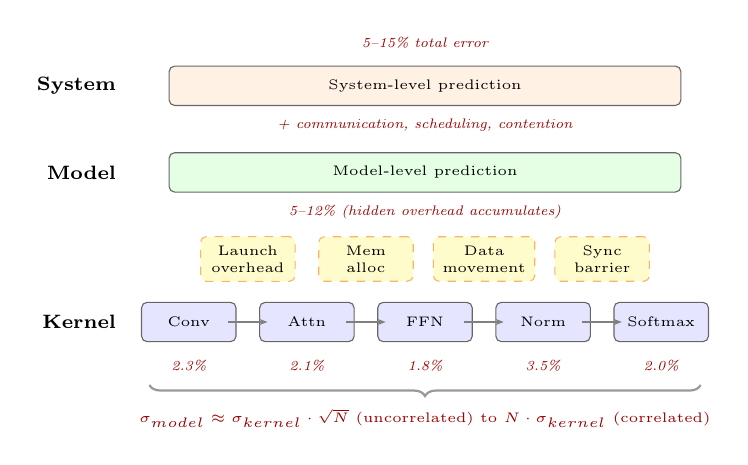
\begin{tikzpicture}[
    box/.style={draw=black!60, rounded corners=2pt, minimum width=1.2cm, minimum height=0.5cm, align=center, font=\tiny},
    err/.style={font=\tiny\itshape, text=red!60!black},
    arr/.style={-{Stealth[length=3pt]}, thick, black!50},
    brace/.style={decorate, decoration={brace, amplitude=4pt, mirror}, thick, black!40},
]

% Kernel level
\node[box, fill=blue!10] (k1) at (0,0) {Conv};
\node[box, fill=blue!10] (k2) at (1.5,0) {Attn};
\node[box, fill=blue!10] (k3) at (3,0) {FFN};
\node[box, fill=blue!10] (k4) at (4.5,0) {Norm};
\node[box, fill=blue!10] (k5) at (6,0) {Softmax};
\node[err] at (0,-0.55) {2.3\%};
\node[err] at (1.5,-0.55) {2.1\%};
\node[err] at (3,-0.55) {1.8\%};
\node[err] at (4.5,-0.55) {3.5\%};
\node[err] at (6,-0.55) {2.0\%};
\node[font=\scriptsize\bfseries, anchor=east] at (-0.8,0) {Kernel};

% Composition arrows
\draw[arr] (0.5,0) -- (1,0);
\draw[arr] (2,0) -- (2.5,0);
\draw[arr] (3.5,0) -- (4,0);
\draw[arr] (5,0) -- (5.5,0);

% Hidden errors
\node[box, fill=yellow!20, dashed, draw=orange!60] (h1) at (0.75,0.8) {Launch\\overhead};
\node[box, fill=yellow!20, dashed, draw=orange!60] (h2) at (2.25,0.8) {Mem\\alloc};
\node[box, fill=yellow!20, dashed, draw=orange!60] (h3) at (3.75,0.8) {Data\\movement};
\node[box, fill=yellow!20, dashed, draw=orange!60] (h4) at (5.25,0.8) {Sync\\barrier};

% Model level
\node[box, fill=green!10, minimum width=6.5cm] (model) at (3,1.9) {Model-level prediction};
\node[err] at (3,1.4) {5--12\% (hidden overhead accumulates)};
\node[font=\scriptsize\bfseries, anchor=east] at (-0.8,1.9) {Model};

% System level
\node[box, fill=orange!10, minimum width=6.5cm] (system) at (3,3.0) {System-level prediction};
\node[err] at (3,2.5) {+ communication, scheduling, contention};
\node[font=\scriptsize\bfseries, anchor=east] at (-0.8,3.0) {System};
\node[err] at (3,3.55) {5--15\% total error};

% Braces
\draw[brace] (-0.5,-0.8) -- (6.5,-0.8) node[midway, below=5pt, font=\tiny, text=red!60!black] {$\sigma_{\text{model}} \approx \sigma_{\text{kernel}} \cdot \sqrt{N}$ (uncorrelated) to $N \cdot \sigma_{\text{kernel}}$ (correlated)};

\end{tikzpicture}%
}
\caption{Error composition across abstraction levels. Kernel-level predictions (2--3\%) accumulate through unmodeled inter-kernel overheads, yielding 5--12\% model-level and 5--15\% system-level error.}
\label{fig:error-composition}
\end{figure}

\textbf{2. Frontier workload coverage.}
The temporal validation lag (Section~\ref{sec:taxonomy}) is closing for transformers but remains wide: MoE, diffusion~\cite{dynamicreasoning2026}, and dynamic inference lack validated tools; scaling laws~\cite{kaplan2020scaling,hoffmann2022chinchilla,scalinglaws2024,scalinglawguide2025} predict loss but not latency.
Figure~\ref{fig:workload-coverage} shows the post-2023 shift toward LLM workloads.

\begin{figure}[t]
\centering
\resizebox{\columnwidth}{!}{%
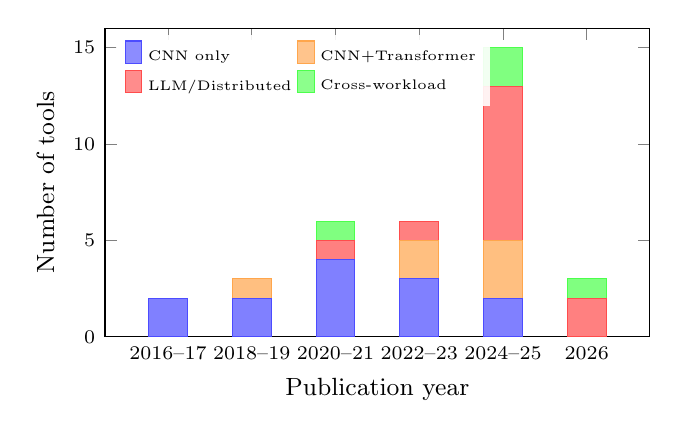
\begin{tikzpicture}
\begin{axis}[
    ybar stacked,
    bar width=14pt,
    xlabel={Publication year},
    ylabel={Number of tools},
    ymin=0, ymax=16,
    xtick={2016,2018,2020,2022,2024,2026},
    xticklabels={2016--17,2018--19,2020--21,2022--23,2024--25,2026},
    xticklabel style={font=\scriptsize},
    yticklabel style={font=\scriptsize},
    xlabel style={font=\small},
    ylabel style={font=\small},
    legend style={at={(0.02,0.98)}, anchor=north west, font=\tiny, draw=none, fill=white, fill opacity=0.9, text opacity=1, legend columns=2},
    legend cell align={left},
    height=5.5cm,
    width=8.5cm,
    enlarge x limits={abs=0.8cm},
]
\addplot[fill=blue!50, draw=blue!70] coordinates {(2016,2) (2018,2) (2020,4) (2022,3) (2024,2) (2026,0)};
\addplot[fill=orange!50, draw=orange!70] coordinates {(2016,0) (2018,1) (2020,0) (2022,2) (2024,3) (2026,0)};
\addplot[fill=red!50, draw=red!70] coordinates {(2016,0) (2018,0) (2020,1) (2022,1) (2024,8) (2026,2)};
\addplot[fill=green!50, draw=green!70] coordinates {(2016,0) (2018,0) (2020,1) (2022,0) (2024,2) (2026,1)};
\legend{CNN only, CNN+Transformer, LLM/Distributed, Cross-workload}
\end{axis}
\end{tikzpicture}%
}
\caption{Workload coverage by publication period. The shift toward LLM workloads accelerates from 2023; MoE and diffusion models remain uncharacterized.}
\label{fig:workload-coverage}
\end{figure}

\textbf{3. Hardware transfer and emerging architectures.}
Cross-family transfer (GPU$\rightarrow$TPU$\rightarrow$PIM) remains unsolved despite meta-learning (HELP) and feature-based transfer (LitePred).
PIM~\cite{upimulator2024,attacc2024,neupims2024,paise2025}, chiplets, and disaggregated designs blur memory hierarchy assumptions that current analytical models rely on.

\textbf{4. Standardized evaluation infrastructure.}
No MLPerf~\cite{mlperf_training2020,mlperf_inference2020} equivalent exists for performance \emph{prediction}.
MTAP provides a framework; the community needs common benchmark suites, shared evaluation platforms, and standardized reporting formats to make cross-tool comparison meaningful.
Portable workload formats (ONNX, Chakra~\cite{chakra2023}) and Docker-first deployment are prerequisites.

\textbf{5. Temporal stability.}
Software stack evolution (FlashAttention~\cite{flashattention2022}, new CUDA versions, framework updates) silently invalidates models.
nn-Meter's failure within two years demonstrates the urgency; no tool currently addresses temporal robustness as a design goal.
Future tools should adopt continuous validation against evolving baselines~\cite{mlperfpower2025}.

% ==============================================================================
% CONCLUSION
% ==============================================================================
\section{Conclusion}
\label{sec:conclusion}

This survey of 22 ML performance modeling tools introduces the Multi-dimensional Tool Assessment Protocol (MTAP), a principled evaluation framework that goes beyond accuracy to assess compositional fidelity, generalization robustness, deployment viability, and extensibility.
Applying MTAP to five tools yields three actionable findings.
First, \emph{structural decomposition aligned with hardware execution boundaries} is the dominant design principle: Timeloop's loop nests for systolic arrays, NeuSight's tiles for GPU SMs, and VIDUR's prefill/decode phases all succeed by matching prediction granularity to hardware scheduling units.
Second, \emph{the composition gap is the field's central unsolved problem}: kernel-level errors (2--3\%) amplify by $5$--$10\times$ at the system level through unmodeled inter-kernel overheads, and no tool provides formal composition guarantees.
Third, \emph{deployment methodology predicts usability better than modeling sophistication}: Docker-first tools remain usable years later, while the tool with the lowest reported error (nn-Meter, $<$1\%) fails to produce any output.
The most pressing needs are standardized evaluation infrastructure (adopting MTAP or similar frameworks), validated tools for frontier workloads, and formal error composition bounds.

%%%%%%% -- PAPER CONTENT ENDS -- %%%%%%%%

%%
%% The next two lines define the bibliography style to be used, and
%% the bibliography file.
\bibliographystyle{ACM-Reference-Format}
\bibliography{references}

\end{document}
